
\section{Results}
\label{sec:results}

As explained in the methodology, the first step is to perform clustering process on the dataset in order to properly label the samples according to the classes to be used in the decision tree algorithm. Figure \ref{fig:clusters} presents a sample of the results obtained after the constrained \kmeans{} clustering process is completed, including subspacing. Recall that there are a total of 550 subspaces. Fig.~\ref{fig:clusters} shows three examples for each one of the types of subspaces, that is, three for each one of the 2-, 3-, and 4-feature analyses. However, since it is not practical or possible to present three- or higher-dimensional plots, we display the results from a two-dimensional perspective into the the subspaces by picking 2 metrics at a time. (Note that in the only cases in which this is a direct view into the clustering results is in the cases of the 2-feature analysis.)

% There are some characteristics of the results shown in Fig.~\ref{fig:clusters} worth 

subspaces for an ordered sequence of metric pairs from C1 to C11 (see Table \ref{tab:metrics}). Although it would be impractical to discuss all the possible combinations, some points can be made from those shown in this figure. For instance, not all feature combinations lead to clearly distinguishable clusters. In this sample we include well-partitioned sets such as C3-C4, C5-C6, C7-C8, and some others where the data-points are mixed across classes, such as subspaces C1-C2 and C10-C11. Note also that although some data distribution may hint the existence of clusters, they may nonetheless be irrelevant because knowledge about one feature does not add insight about the other. That is the case of the C9-C10 subspace. Conversely, there are subspaces with a clear correlation between the data, but with indistinguishable clusters. That is the case of the C1-C2 subspace. These latter two types of subspaces do not contribute information to the clustering process \citep{Dy_2004_MLR}. 

\begin{figure*}[ht!]
	\centering
	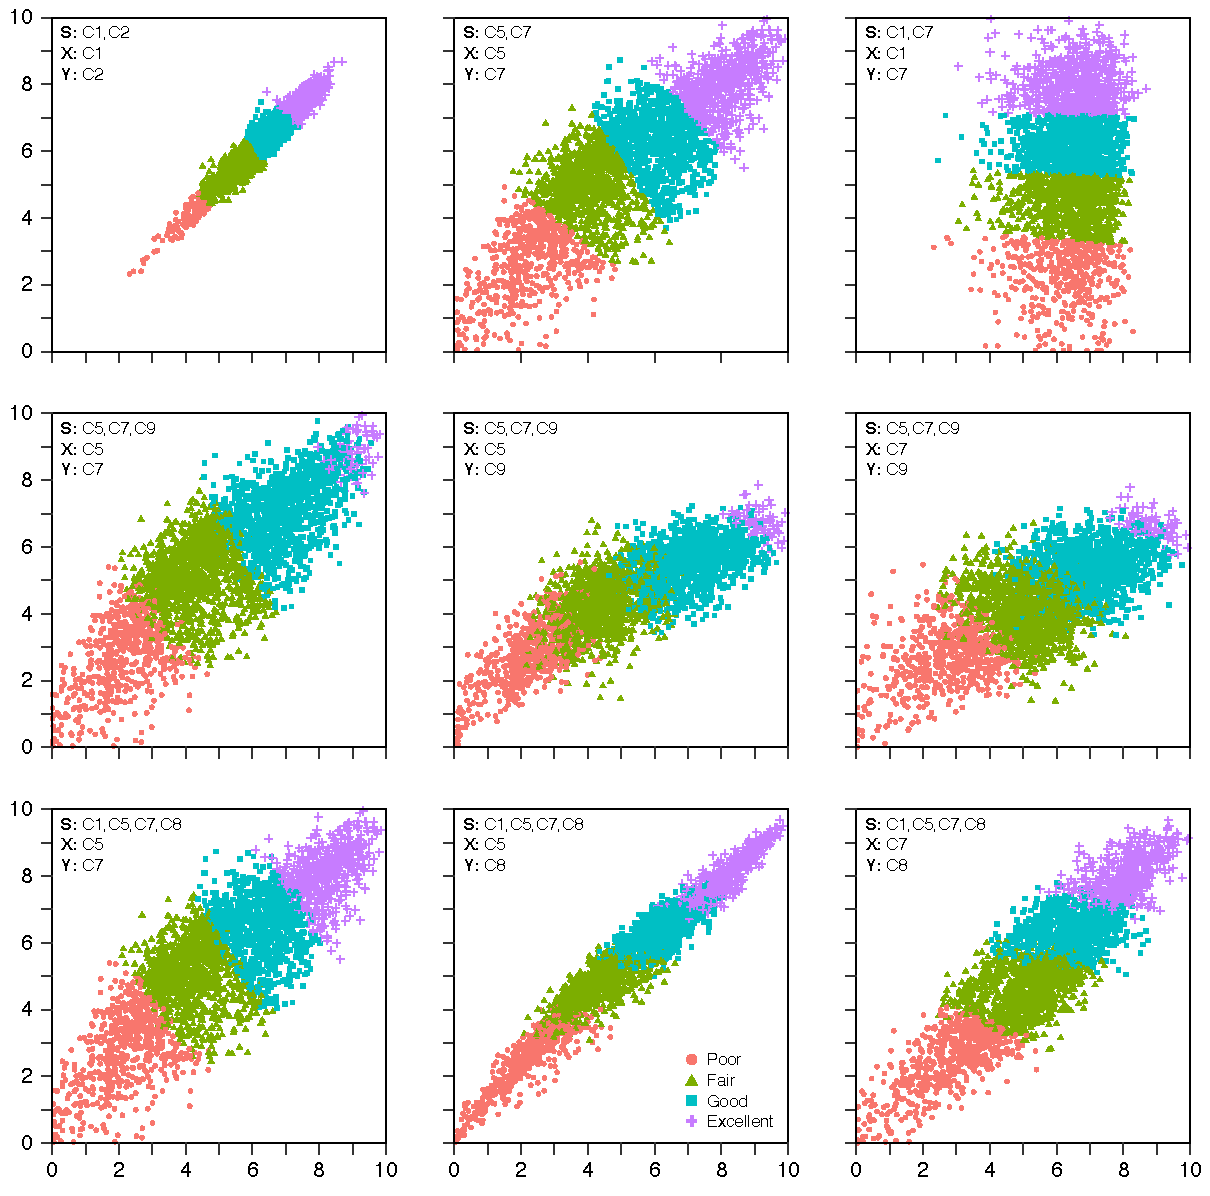
\includegraphics[width=\textwidth]{figures/pdf/figure-05}
	\caption{A sample of the results from the multi-dimensional clustering analysis for pairs of consecutive metrics C1 through C11. These results are part of the 55 possible sub-spaces with 2 features (metrics). The cluster centers are shown with a cross symbol. Although for some pairs it may be obvious, the clusters 1 through 4 do not necessarily correspond in that order to the validation classes poor, fair, good, and excellent. The color version of this figure is available only in the electronic edition.}
	\label{fig:clusters}
\end{figure*}

Figure \ref{fig:boxed-clusters} shows the statistical distribution of the data in the form of box-plots for each metric and component of motion once partitioned into the four validation classes. Separately, we have prepared similar plots for the different velocity models used in the simulations from where we obtained our dataset. As in Fig.~\ref{fig:data-box-plot} before the clustering, and in Fig.~\ref{fig:data-box-plot} after the clustering process, we observe that the velocity models and the components of motion do not have a strong influence on the statistical distribution of the data, that is why we merge all the data samples into a single dataset at the before processing the data and we continue forward with that approach after clustering and labeling.

In total, the initial dataset is partitioned into groups of 816, 1253, 879 and 76 data samples for the poor, fair, good and excellent classes, respectively. These groups are shown in Fig.~\ref{fig:count-classes}, which also show the contribution of the component of motion to the final count of samples in each class for illustrative purposes. The main aspect to notice in this figure and the quantities just provided is the fact that the number of samples in the excellent class is significantly less than those of the poor, fair, and good classes. 

\begin{figure*}
	\centering
	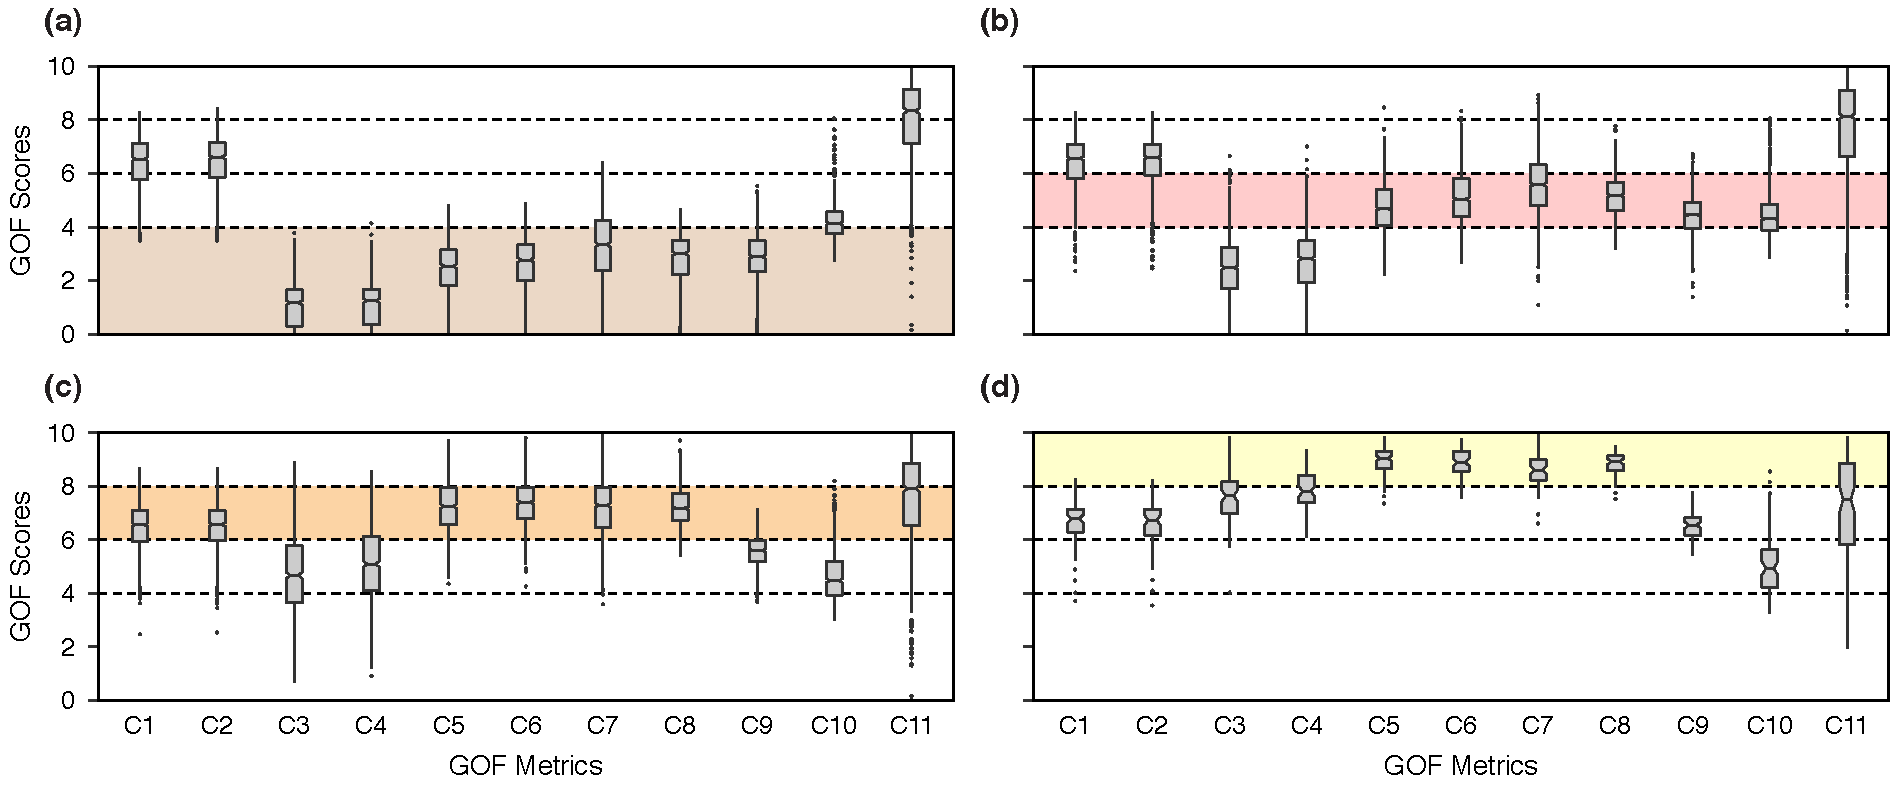
\includegraphics[width=\textwidth]{figures/pdf/figure-06}
	\caption{Statistical distribution of the dataset as partitioned into the four validation categories (poor, fair, good, excellent) after the clustering analysis. The distributions are shown in the form of box-plots for each metric (C1 through C11), and discretized in terms of the component of motion (NS, EW, UD) for visualization purposes. In each case, the median is indicated by a notch in the box of the central quartiles, and the lines represent the interquartile range, with outliers shown as scattered dots. The color version of this figure is available only in the electronic edition.}
	\label{fig:boxed-clusters}
\end{figure*}

As a consequence, before moving on with the decision tree analysis, it is necessary to do resampling on the subset of the excellent class. In order to maintain a good number of samples for the other three classes, we used the oversampling approach described in the previous section. To that end, we replicated data randomly by a $\times$10 factor until elevating the number of samples in this class to 760 as indicated in Fig.~\ref{fig:count-classes}. By common standards, an oversample rate of $\times$10 is considered acceptable \citep{Weiss_2003_JAIR}. (Arguably, we could have as well undersampled the fair class, but we deemed that unnecessary.) Once this process was completed we went on with the decision tree analysis. 

\begin{figure}[t]
	\centering
	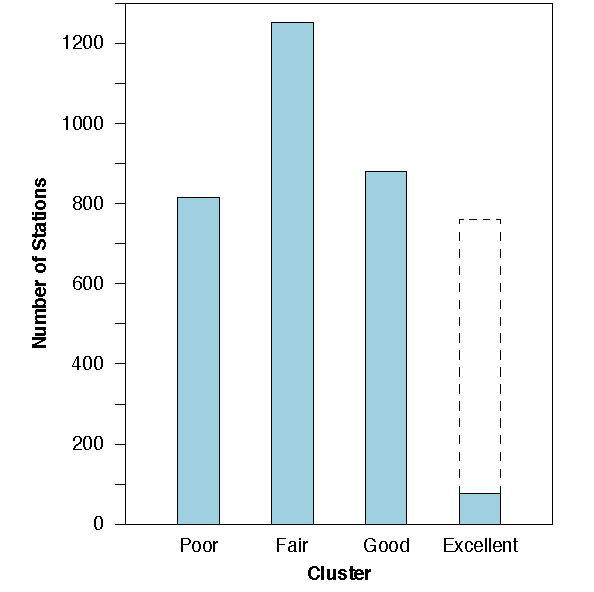
\includegraphics[width=\columnwidth]{figures/pdf/figure-07}
	\caption{Number of data samples in each class (poor, far, good, excellent) after conducting a multi-dimensional constrained \kmeans{} clustering process using subspace analysis for 2, 3, and 4 features (GOF metrics). Here, for illustrative purposes, the filling of the bars distinguishes the component of motion of the compared signals as classified. The dashed-line bar indicates the number of samples in the excellent class after oversampling.}
	\label{fig:count-classes}
\end{figure}

In total we generated 20,000 trees using the C5.0 algorithm for combinations of the parameters CF and $S_{\min}$. CF was chosen to vary between 0 and 1 at intervals of size 0.01, and $S_{\min}$ between 1 and 200 at unitary intervals. Not surprisingly, for such a small size intervals, the algorithm often reached the same tree for different CF and $S_{\min}$ values. Therefore, in reality, from the 20,000 we ran the algorithm, we only found 66 unique trees. For each one of these unique threes, we computed the effectiveness factor $F_1$ from equation (\ref{eq:f}) and extracted the total number of nodes in the trees and their depth.

Figure... (working)


